\documentclass[border=0.125cm]{standalone}
\usepackage{tikz}
\usepackage{ifthen}
\usetikzlibrary{matrix,chains,positioning,decorations.pathreplacing,arrows}
\usetikzlibrary{positioning,calc}
\begin{document}

\tikzset{%
  every neuron/.style={
    circle,
    draw,
    minimum size=1cm
  },
  neuron missing/.style={
    draw=none,
    scale=4,
    text height=0.333cm,
    execute at begin node=\color{black}$\vdots$
  },
}

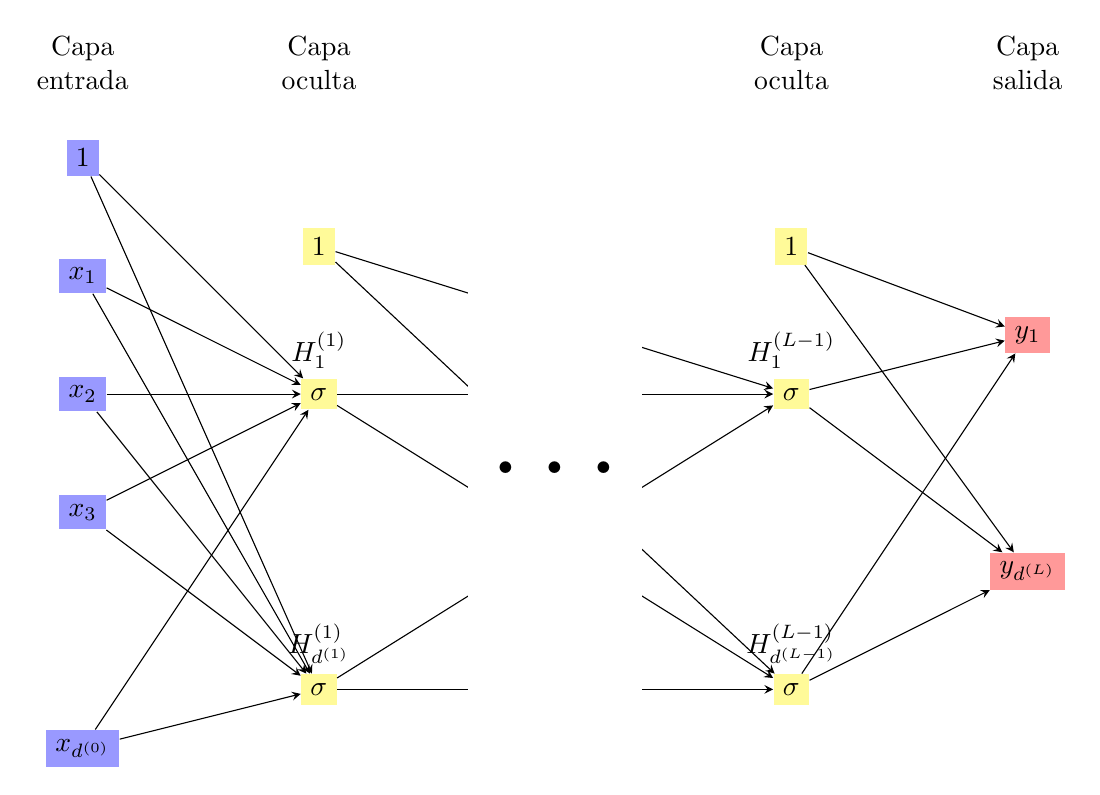
\begin{tikzpicture}[x=1.5cm, y=1.5cm, >=stealth]

\foreach \m/\l [count=\y] in {0,1,2,3,missing,4}
  \ifthenelse{\equal{\m}{missing}}{\node [every neuron/.try, neuron \m/.try] (input-\m) at (0,2.5-\y){}}{\node [every neuron/.try, neuron \m/.try, fill=blue!40] (input-\m) at (0,2.5-\y) {\ifthenelse{\equal{\m}{missing}}{}{\ifthenelse{\equal{\m}{4}}{$x_{d^{(0)}}$}{\ifthenelse{\equal{\m}{0}}{1}{$x_\m$}}}}};

\foreach \m [count=\y] in {0,1,missing,2}
  \ifthenelse{\equal{\m}{missing}}{\node [every neuron/.try, neuron \m/.try ] (hidden1-\m) at (2,2-\y*1.25){}}{\node [every neuron/.try, neuron \m/.try, fill=yellow!40] (hidden1-\m) at (2,2-\y*1.25) {\ifthenelse{\equal{\m}{missing}}{}{\ifthenelse{\equal{\m}{0}}{1}{$\sigma$}}}};

\foreach \m [count=\y] in {0,1,missing,2}
  \ifthenelse{\equal{\m}{missing}}{\node [every neuron/.try, neuron \m/.try ] (hidden2-\m) at (6,2-\y*1.25){}}{\node [every neuron/.try, neuron \m/.try, fill=yellow!40] (hidden2-\m) at (6,2-\y*1.25) {\ifthenelse{\equal{\m}{missing}}{}{\ifthenelse{\equal{\m}{0}}{1}{$\sigma$}}}};

\foreach \m [count=\y] in {1,missing,2}
  \ifthenelse{\equal{\m}{missing}}{\node [every neuron/.try, neuron \m/.try ] (output-\m) at (8,1-\y){}}{\node [every neuron/.try, neuron \m/.try, fill=red!40] (output-\m) at (8,1-\y) {\ifthenelse{\equal{\m}{missing}}{}{\ifthenelse{\equal{\m}{2}}{$y_{d^{(L)}}$}{$y_\m$}}}};

\foreach \l [count=\i] in {1,d^{(1)}}
  \node [above] at (hidden1-\i.north) {$H_{\l}^{(1)}$};

\foreach \l [count=\i] in {1,d^{(L-1)}}
  \node [above] at (hidden2-\i.north) {$H_{\l}^{(L-1)}$};

\foreach \i in {0,...,4}
  \foreach \j in {1,...,2}
    \draw [->] (input-\i) -- (hidden1-\j);

\foreach \i in {0,...,2}
  \foreach \j in {1,...,2}
    \draw [->] (hidden1-\i) -- (hidden2-\j);

    \foreach \i in {0,...,2}
    \foreach \j in {1,...,2}
    \draw [->] (hidden2-\i) -- (output-\j);

\node [align=center, above] at (0,2) {Capa\\entrada};
\node [align=center, above] at (2,2) {Capa \\oculta};
\node [align=center, above] at (6,2) {Capa \\oculta};
\node [align=center, above] at (8,2) {Capa \\salida};

\node[fill=white,scale=4,inner xsep=2pt,inner ysep=8mm] at ($(hidden1-0)!.5!(hidden2-2)$) {$\dots$};

\end{tikzpicture}
\end{document}
